%%%%%%%%%%%%%%%%%%%%%%%%%%%%%%%%% LAB-5 %%%%%%%%%%%%%%%%%%%%%%%%%%%%%%%%%%
%>>>>>>>>>>>>>>>>>>>>>>>>>> ПЕРЕМЕННЫЕ >>>>>>>>>>>>>>>>>>>>>>>>>>>>>>>>>>>
%>>>>> Информация о кафедре
%\newcommand{\year}{2021 г.}  % Год устанавливается автоматически
\newcommand{\city}{Санкт-Петербург}  %  Футер, нижний колонтитул на титульном листе
\newcommand{\university}{Национальный исследовательский университет ИТМО}  % первая строка
\newcommand{\department}{Факультет программной инженерии и компьютерной техники}  % Вторая строка
\newcommand{\major}{Направление системного и прикладного программного обеспечения}  % Треьтя строка
%<<<<< Информация о кафедре

%>>>>> Назание работы
\newcommand{\reporttype}{ОТЧЕТ ПО ЛАБОРАТОРНОЙ РАБОТЕ} % тип работы, (главный заголовок титульного листа)
\newcommand{\lab}{Лабораторная работа}          % вид работы
\newcommand{\labnumber}{№ 1}                    % порядковый номер работы
\newcommand{\subject}{Функциональная схемотехника}         % учебный предмет
\newcommand{\labtheme}{Ведение в проектирование цифровых интегральных схем}            % Тема лабораторной работы
\newcommand{\variant}{№ 6}                % номер варианта работы

\newcommand{\student}{Тюрин Иван Николаевич}    % определение ФИО студента
\newcommand{\studygroup}{P33102}                 % определение учебной группы 
\newcommand{\teacher}{% принимающий
    Кустарев П. В.,\\[1mm]% ФИО лектора
    Васильев С.Е.% ФИО практика
}
%<<<<<<<<<<<<<<<<<<<<<<<<<< ПЕРЕМЕННЫЕ <<<<<<<<<<<<<<<<<<<<<<<<<<<<<<<<<<<


%>>>>>>>>>>>>>>>>>>>>>> ПРЕАМБУЛА >>>>>>>>>>>>>>>>>>>>>>>>>

%>>>>>>>>>>>>>>>>>> ПРЕАМБУЛА >>>>>>>>>>>>>>>>>>>>
\documentclass[14pt,final,oneside]{extreport}% класс документа, характеристики
%>>>>> Разметка документа
\usepackage[a4paper, mag=1000, left=3cm, right=1.5cm, top=2cm, bottom=2cm, headsep=0.7cm, footskip=1cm]{geometry} % По ГОСТу: left>=3cm, right=1cm, top=2cm, bottom=2cm,
\linespread{1} % межстройчный интервал по ГОСТу := 1.5
%<<<<< Разметка документа

%>>>>> babel c языковым пакетом НЕ должны быть первым импортируемым пакетом
\usepackage[utf8]{inputenc}
\usepackage[T1,T2A]{fontenc}
\usepackage[russian]{babel}
%<<<<<

%\usepackage{cmap} %поиск в pdf

%>>>...>> прочие полезные пакеты
\usepackage{amsmath,amsthm,amssymb}
\usepackage{mathtext}
\usepackage{indentfirst}
\usepackage{graphicx}
\usepackage{float}
\graphicspath{{/home/ivan/itmo/informatics/latex}}
\DeclareGraphicsExtensions{.pdf,.png,.jpg}
%\usepackage{bookmark}

\usepackage[dvipsnames]{xcolor}
\usepackage{hyperref}  % Использование ссылок
\hypersetup{%  % Настройка разметки ссылок
    colorlinks=true,
    linkcolor=blue,
    filecolor=magenta,      
    urlcolor=magenta,
    %pdftitle={Overleaf Example},
    %pdfpagemode=FullScreen,
}

\usepackage{diagbox}
\usepackage[letterspace=150]{microtype} % Спэйсинг (межбуквенный интервал для саголовка) \lsstyle
% \usepackage{csvsimple} %импорт содержимого таблицы из csv

%>>> верстка в 2 колонки
\usepackage{multicol} % многоколоночная верстка
\setlength{\columnsep}{.15\textwidth} % определение ширины разделителя между колонками

\usepackage{tikz} % пакет для векторной графики, чтобы рисовать красивый разделитель колонок
% %> кастомный разделитель колонок
% \usetikzlibrary{arrows.meta,decorations.pathmorphing,backgrounds,positioning,fit,petri}
% \usepackage{multicolrule} % Для кастомизации разделителя колонок
% \SetMCRule{                     % кастомизация разделителя колонок multicolrule
%     width=2pt,
%     custom-line={               % Tikz код для кастомизации линии разделителя
%         \draw [                 % Рисовать
%             decorate,           % декорированную (требуются спец настройки пакетов tikz (см. импорт выше)
%             decoration={        % вид декорирования
%                 snake, % Тип - змейка (волнистая)
%                 amplitude=.5mm, % ширина волн
%                 pre length=0mm, % участок прямой линии от начала
%                 %segment length=0mm, % учасок волнистой линии
%                 post length=0mm % участок прямой линии от конца
%             },
%             line width=1pt,
%             step=10pt
%         ] 
%         (TOP) to (BOT); % сверху и до низа колонки
%     }, 
%     extend-top=-5pt, % Вылезти за верхнюю границу колонки 
%     extend-bot=-7pt % Вылезти за нижнюю границу колонки  
% }
%% < кастомный разделитель колонок
%%<<< верстка в 2 колонки

%>>>>> Использование листингов
\usepackage{listings} 
\usepackage{caption}
\DeclareCaptionFont{white}{\color{white}} 
\DeclareCaptionFormat{listing}{\colorbox{gray}{\parbox{\textwidth}{#1#2#3}}}

\captionsetup[lstlisting]{format=listing,labelfont=white,textfont=white} % Настройка вида описаний
\lstset{  % Настройки вида листинга
inputencoding=utf8, extendedchars=\true, keepspaces = true, % поддержка кириллицы и пробелов в комментариях
language={},            % выбор языка для подсветки (здесь это Pascal)
basicstyle=\small\sffamily, % размер и начертание шрифта для подсветки кода
numbers=left,               % где поставить нумерацию строк (слева\справа)
numberstyle=\tiny,          % размер шрифта для номеров строк
stepnumber=1,               % размер шага между двумя номерами строк
numbersep=5pt,              % как далеко отстоят номера строк от подсвечиваемого кода
backgroundcolor=\color{white}, % цвет фона подсветки - используем \usepackage{color}
showspaces=false,           % показывать или нет пробелы специальными отступами
showstringspaces=false,     % показывать илигнет пробелы в строках
showtabs=false,             % показывать или нет табуляцию в строках
frame=single,               % рисовать рамку вокруг кода
tabsize=2,                  % размер табуляции по умолчанию равен 2 пробелам
captionpos=t,               % позиция заголовка вверху [t] или внизу [b] 
breaklines=true,            % автоматически переносить строки (да\нет)
breakatwhitespace=false,    % переносить строки только если есть пробел
escapeinside={\%*}{*)}      % если нужно добавить комментарии в коде
}

\definecolor{codegreen}{rgb}{0,0.6,0}
\definecolor{codegray}{rgb}{0.5,0.5,0.5}
\definecolor{codepurple}{rgb}{0.58,0,0.82}
\definecolor{backcolour}{rgb}{0.97,0.97,0.97}

\lstdefinestyle{mystyle}{
    backgroundcolor=\color{backcolour},   
    commentstyle=\color{codegreen},
    keywordstyle=\color{magenta},
    numberstyle=\tiny\color{codegray},
    stringstyle=\color{codepurple},
    basicstyle=\ttfamily\footnotesize,
    breakatwhitespace=false,         
    breaklines=false,                 
    captionpos=b,                    
    keepspaces=true,                 
    numbers=left,                    
    numbersep=5pt,                  
    showspaces=false,                
    showstringspaces=false,
    showtabs=false,                  
    tabsize=2
}
\lstset{style=mystyle}
%<<<<< Использование листингов


\sloppy % Решение проблем с переносами (с. 119 книга Львовского)
\emergencystretch=25pt


%>>>>>>>>>>>>>>>> ДОПОЛНИТЕЛЬНЫЕ КОМАНДЫ {Для соответствия ГОСТ} >>>>>>>>>>>>>>
%>>>>>> математические функции для удобства
\newcommand{\tx}{\text}
\newcommand{\eps}{\varepsilon}
\renewcommand{\phi}{\varphi}
\newcommand{\limit}{\displaystyle\lim}
\newcommand{\oo}{\infty}
\newcommand{\De}{\Delta}
\newcommand{\cd}{\cdot}
\newcommand{\df}{\partial}
\newcommand{\ndash}{\textendash}
\newcommand{\mdash}{\textemdash}

%>>>>> Аннотирование
\newcommand{\note}[2]{\overbrace{#1}^{#2}}% скобка сверху для комментария
% \overset{}{}% для указания символа над другим смиволом
% \underset{}{}% для указания символа под другим смиволом
%<<<<< Аннотирование

%>>>>>> Матрицы
\DeclareMathOperator{\rank}{rank}
\newcommand{\tvec}[1]{\mathbfit{#1}}% "text vector"
\newcommand{\mtx}[1]{\mathrm{#1}}
\newcommand{\transposed}[1]{{#1}^{\mathrm{T}}}
%>>>>>> Матрицы

%>>>>> Скобки
\newcommand{\lt}{\left}
\newcommand{\rt}{\right}
\newcommand{\la}{\langle}% '<'
\newcommand{\ra}{\rangle}% '>'
\newcommand{\avg}[1]{\langle{#1}\rangle}% '<X>'
%<<<<< Скобки

%>>>>> Дроби
\newcommand{\cf}[2]{\cfrac{#1}{#2}}
\newcommand{\fr}[2]{\frac{#1}{#2}}
%<<<<< Дроби


%>>>>> Стрелки
\newcommand{\Rarr}{\Rightarrow}% ⇒ следствие | лучше использовать \implies
\newcommand{\LRarr}{\Leftrightarrow}% равносильно | лучше  использовать \iff
\newcommand{\rarr}{\xrightarrow{}}% → стрелка вправо
\newcommand{\nwarr}{\nwarrow}% ↖ север-запад стрелка
\newcommand{\nearr}{\nearrow}% ↗ север-восток стрелка
\newcommand{\swarr}{\swarrow}% ↙ юг-запад стрелка
\newcommand{\searr}{\searrow}% ↘ юг-восток стрелка

\newcommand{\raises}{\nwarrow}% возрастает
\newcommand{\increases}{\nwarrow}% возрастает
\newcommand{\falls}{\swarrow}% убывает
\newcommand{\decreases}{\swarrow}% убывает

%{{{
\makeatletter
\newcommand{\impliesby}[2][]{\ext@arrow 0359\Leftrightarrowfill@{#1}{#2}}% следствие с надписью
\makeatother
%}}}

%{{{
\makeatletter
\newcommand{\iffby}[2][]{\ext@arrow 0359\Rightarrowfill@{#1}{#2}}% равносильность с надписью
\makeatother
%}}}
%<<<<< Стрелки

% Функции для удобного описания формул: https://tex.stackexchange.com/questions/95838/how-to-write-a-perfect-equation-parameters-description



%<<<<<< математические функции для удобства
%>>>>>> Стиль текста
\newcommand{\hex}[1]{\texttt{0{\footnotesize{x}}#1}}
\newcommand{\ttt}[1]{\texttt{#1}}
%<<<<<< Стиль текста

\newcommand\Chapter[3]{%
    % Принимает 3 аргумента - название главы и дополнительный заголовок и множитель ширины загловка (можно ничего)
    \refstepcounter{chapter}%
    \chapter*{%
        %\hfill % заполнение отступом пространства до заголовка
        \begin{minipage}{#3\textwidth} % Можно изменить ширину министраницы (заголовка)
            \flushleft % Выранивание заголовка по левому краю параграфа (заголовка)
            %\flushright % Выранивание заголовка по правому краю параграфа (заголовка)
            \begin{huge}%
                % Отключена нумерация глав в тексте:
                % \textbf{\chaptername\ \arabic{chapter}\\}
                \textbf{#1}% Первый заголовок
            \end{huge}%
            \\% Перенос сторки
            \begin{Huge}
                #2% Второй заголовок
            \end{Huge}
        \end{minipage}
    }%
    % Отключена нумерация для chapter в toc (table of contents), т.е. Оглавлении (Содержании):
    % \addcontentsline{toc}{chapter}{\arabic{chapter}. #1}
    % Представление главы в содержании:
    \addcontentsline{toc}{chapter}{#1. #2}%
}

\newcommand\Section[1]{
    % Принимает 1 аргумент - название секции
    \refstepcounter{section}
    \section*{%
        \raggedright
        % Отключена дополнительная нумерация chapter в section в тексте документа:
        % \arabic{chapter}.\arabic{section}. #1}
        % Отключена любая нумарация section в тексте документа: 
        \arabic{section}. #1%
    }
    
    % Отключена дополнительная нумерация chapter в section в toc (table of contents) Оглавлении (Содержании):
    % \addcontentsline{toc}{section}{\arabic{chapter}.\arabic{section}. #1}
    \addcontentsline{toc}{section}{\arabic{section}. #1} 
}


\newcommand\Subsection[1]{
    % Принимает 1 аргумент - название подсекции
    \refstepcounter{subsection}
    \subsection*{%
        \raggedright%
        % Отключена дополнительная нумерация chapter в section в тексте документа (можно добавить отступ с помощью \hspace*{12pt}):
        % \arabic{chapter}.\arabic{section}.\arabic{subsection}. #1}
        \arabic{section}.\arabic{subsection}. #1
    }
    % Отключена дополнительная нумерация chapter в section в Оглавлении (Содержании):
    %\addcontentsline{toc}{subsection}{\arabic{chapter}.\arabic{section}.\arabic{subsection}. #1}
    \addcontentsline{toc}{subsection}{\arabic{subsection}. #1}
}


\newcommand\Figure[4]{
    % Принимает 4 аргумента - название файла изображения, ее размер в тексте, описание, лэйбл (псевдоним в формате "fig:name") 
    %
    \refstepcounter{figure}
    \begin{figure}[H] %- \usepackage {float} %[h]
        \begin{center}
            \fbox{
                \includegraphics[width=#2]{#1}
            }
        \end{center}
        \begin{center}
            Рис.~\arabic{figure}. #3.
        \end{center}
        %\caption{#3}
        \label{fig:#4}
    \end{figure}
}


\newcommand\Table[3]{
    % Принимает 3 аргумента --- лэйбл name(#1) (псевдоним в формате "tab:name"), ее описание(#2), содержание таблицы(#3)
    % ВАЖНО!: от этого способа страдает нумерация описаний, можно использовать создание таблиц через googlesheet
    %
    \renewcommand{\arraystretch}{1.2} % Установка высоты строки таблицы по умолчанию, увеличенное на 0.2 пункта
    % \refstepcounter{table}% увеличение счетчика таблиц
    \begin{table}[Htpb]% "right Here", "top", "new page", "bottom"
        \label{tab:#1}% лэйбл таблицы, для ссылок
        \resizebox{\columnwidth}{!}{% сжимает очень широкие таблицы, чтобы вместить на страницу
             #3% Содержимое таблицы
        }
        % 
        \caption{#2}% Описание стандартными средствами для используемого окружения (table)
        % \captionof{table}{#2}% Описание стандартными средствами
        % \captionof*{figure}{\flushleft \textsc\textbf{Рис. 1.}}% Описание стандартными средствами, как рисунка
        %
        %%> кастомное описание
        % \begin{flushleft}% Кастомное описание
        %     % \textsf{%
        %         \textbf{%
        %             \\[2mm]
        %             #2% Описание к картинке
        %         }%
        %         % \\[8mm]% Отступ
        %     % }%
        % \end{flushleft}
        %%< кастомное описание
    \end{table}
    \renewcommand{\arraystretch}{1} % возврат установка высоты строки таблицы по умолчанию на 1
}


\newcommand\CustomFigure[4]{ % multicols не умеют в table и figure, поэтому приходится извращаться % вставка таблицы с меткой рисунка
    % Принимает 4 аргумента - название файла изображения, ее размер в тексте, описание, лэйбл (псевдоним в формате "fig:name") 
    %
    \refstepcounter{figure}
    \begin{figure}[ht]% "here", "top"
        \begin{center}
            \includegraphics[width=#2]{#1}
        \end{center}
        %
        %\caption{#3}
        \captionof{figure}{#3}% описание стандартными средствами
        % \begin{center}
        \begin{flushleft} % Кастомное описание
            \textbf{%
                #3% Текст описания
            }
        \end{flushleft}
        % \end{center}
        %
        \label{fig:#4}% Лэйбл, для ссылок
    \end{figure}
}


\newcommand\CustomTableFigure[3]{% multicols не умеют в table и figure, поэтому приходится извращаться % вставка таблицы с меткой рисунка
    %
    % Принимает 3 аргумента --- лэйбл name(#1) (псевдоним в формате "tab:name"), ее описание(#2), содержание таблицы(#3) 
    %
    \begin{center}
        \refstepcounter{figure}
        \label{tab:#1}% лэйбл таблицы, для ссылок
        \resizebox{\columnwidth}{!}{% сжимает очень широкие таблицы, чтобы вместить на страницу
            #3% Содержание таблицы
        }
        % 
        \captionof{figure}{#2}% Описание стандартными средствами
        % \captionof*{figure}{\flushleft \textsc\textbf{Рис. 1.}}% Описание стандартными средствами
        %
        \begin{flushleft}% Кастомное описание
            % \textsf{%
                \textbf{%
                    \\[2mm]
                    #2% Описание к картинке
                }%
                % \\[8mm]% Отступ
            % }%
        \end{flushleft}
    \end{center}
}


\newcommand{\InkscapeFigure}[4]{% Вставки иллюстраций из Inkscape (pdf+latex)
    %
    % Принимает 4 параметра: #1 название файла, #2 описание, #3 лейбл #4 размер
    %
    % \begin{minipage}{#4}
        \begin{figure}[htbp]
            \centering
            \def\svgwidth{#4}
            \import{./figures/}{#1.pdf_tex}
            \caption{#2}
            \label{fig:#3}
        \end{figure}
    % \end{minipage}
}


\newcommand\Equation[3]{% Кастомное оформление выражений
    %
    % Принимает 3 аргумента --- лэйбл name (#1) (псевдоним в формате "tab:name"), его описание(#2), содержание выражения (#3) 
    %
    \textbf{#2}% описание
    \begin{equation}
        #3% содержимое выражений
        \label{eq:#1}% лэйбл
    \end{equation}
}

%<<<<<<<<<<<<<<<<<<<<<<<<<<<< ДОПОЛНИТЕЛЬНЫЕ КОМАНДЫ <<<<<<<<<<<<<<<<<<<<<<<<<<

%<<<<<<<<<<<<<<<<<<<<<< ПРЕАМБУЛА <<<<<<<<<<<<<<<<<<<<<<<<<



%%%%%%%%%%%%%%%%%%% СОДЕРЖИМОЕ ОТЧЕТА %%%%%%%%%%%%%%%%%%%%%
%>>>>>>>>>>>>>>> ''''''''''''''''''''''' >>>>>>>>>>>>>>>>>>
\begin{document}


%>>>>>>>>>>>>>>>> ОПРЕДЕЛЕНИЕ НАЗВАНИЙ >>>>>>>>>>>>>>>>>>>>
% Переоформление некоторых стандартных названий
%\renewcommand{\chaptername}{Лабораторная работа}
\renewcommand{\chaptername}{\lab\ \labnumber} % переименование глав
\def\contentsname{Содержание} % переименование оглавления
%<<<<<<<<<<<<<<<< ОПРЕДЕЛЕНИЕ НАЗВАНИЙ <<<<<<<<<<<<<<<<<<<<
% \setlength{\itemsep}{0pt} % установка расстояния между строчками в списках можно использовать локально внутри списка списке
% \setlength{\parskip}{0pt} % 
% \setlength{\parsep}{0pt}  % 

%>>>>>>>>>>>>>>>>> ТИТУЛЬНАЯ СТРАНИЦА >>>>>>>>>>>>>>>>>>>>>
%>>>>>>>>>>>>>>>>>>> ТИТУЛЬНЫЙ ЛИСТ >>>>>>>>>>>>>>>>>>>>>>>
\begin{titlepage}

    % Название университета
    \begin{center}
    \textsc{%
        \university\\[5mm]
        \department\\[2mm]
        \major\\
    }

    \vfill
    \vfill
    % Название работы
    \textbf{\reporttype\ \labnumber\\[3mm]
    курса <<\subject>> \\[6mm]
    по теме: <<\labtheme>>\\[3mm]
    Вариант \variant\\[20mm]
    }
    \end{center}


\hfill
% Информация об авторе работы и проверяющем
\begin{minipage}{.5\textwidth}
    \begin{flushright}
        
            
        Выполнил студент:\\[2mm] 
        \student\\[2mm]
        группа: \studygroup\\[5mm]

        Преподаватель:\\[2mm] 
        \teacher

    \end{flushright}
\end{minipage}

\vfill

    % Нижний колонтитул первой страницы
    \begin{center}
        \city, \the\year\,г.
    \end{center}

\end{titlepage}
%<<<<<<<<<<<<<<<<<<< ТИТУЛЬНЫЙ ЛИСТ <<<<<<<<<<<<<<<<<<<<<<<


%<<<<<<<<<<<<<<<<< ТИТУЛЬНАЯ СТРАНИЦА <<<<<<<<<<<<<<<<<<<<<


%>>>>>>>>>>>>>>>>>>>>> СОДЕРЖАНИЕ >>>>>>>>>>>>>>>>>>>>>>>>>
% Содержание
\tableofcontents
%<<<<<<<<<<<<<<<<<<<<< СОДЕРЖАНИЕ <<<<<<<<<<<<<<<<<<<<<<<<<


%%%%%%%%%%%%%%%%%%%%%%% КОД РАБОТЫ %%%%%%%%%%%%%%%%%%%%%%%%
%>>>>>>>>>>>>>>>>>>>'''''''''''''''''>>>>>>>>>>>>>>>>>>>>>
\newpage
\Chapter{\lab\ \labnumber}{\labtheme}{}
\Section{Цели работы}
\begin{enumerate}
    \item Получить базовые знания о принципах построения цифровых интегральных схем с использованием технологии КМОП.
    \item Познакомиться с технологией SPICE-моделирования схем на транзисторах.
    \item Получить навыки описания схем базовых операционных элементов (БОЭ) комбинационного типа на вентильном уровне с использованием языка описания аппаратуры Verilog HDL.
\end{enumerate}

\Section{Задание варианта \variant}

% \begin{center} , , , \end{center}
\Subsection{Часть 1}
\begin{enumerate}
    \item Постройте в LTspice на транзисторах схему вентиля, составляющего основу логического базиса согласно варианту задания.
    \item Создайте символ для разработанного вентиля как иерархического элемента.
    \item С использованием созданного иерархического элемента постройте схему тестирования вентиля.
    \item Проведите моделирование работы схемы и определите задержку распространения сигнала через тестируемый вентиль.
    \item Определите максимальную частоту изменения входных сигналов, при которой построенная схема сохраняет работоспособность.
    \item Постройте БОЭ на базе созданного вентиля согласно варианту задания.
    \item Создайте символ для построенного БОЭ.
    \item Проведите моделирование работы схемы и определите задержку распространения сигнала через БОЭ.
    \item Определите максимальную частоту изменения входных сигналов, при которой
построенная схема сохраняет работоспособность.
    \item Составьте отчет по результатам выполнения заданий первой части лабораторной работы.
\end{enumerate}

\Subsection{Часть 2}
\begin{enumerate}
    \item Опишите на Verilog HDL на вентильном уровне модуль, реализующий функцию БОЭ в указанном логическом базисе согласно варианту задания.
    \item Разработайте тестовое окружение для созданного модуля.
    \item Проведите моделирование работы схемы.
    \item Составьте отчет по результатам выполнения заданий второй части лабораторной работы.
\end{enumerate}

Вариант:  
\begin{table}[htb]
    \centering
    \begin{tabular}{|c|c|c|}\hline
        №  варианта & Логический базис  & БОЭ \\\hline
        6           & NAND              & Позиционный дешифратор «3 в 8»\\\hline
    \end{tabular}
    \caption{Вариант задания}
    \label{tab:variant}
\end{table}

% Отчет должен включать:
% 1. Титульный лист.
% 2. Цели работы.
% 3. Задание в соответствии с вариантом.
% 4. Отчет о выполнении заданий части 1:
% − схема разработанного вентиля;
% − символ вентиля и схема тестирования;
% − временная диаграмма процесса тестирования вентиля;
% − результат измерения задержки распространения сигнала через вентиль;
% − максимальная частота работы вентиля;
% − схема разработанного БОЭ;
% − символ разработанного БОЭ и схема тестирования;
% − временная диаграмма процесса тестирования БОЭ;
% − результат измерения задержки распространения сигнала через БОЭ;
% − максимальная частота работы БОЭ.
% 5. Отчет о выполнении заданий части 2:
% − код разработанного модуля БОЭ;
% − код разработанного тестового окружения БОЭ;
% − временная диаграмма процесса тестирования БОЭ.
% 6. Выводы по работе.


% \begin{itemize}
%     \setlength{\itemsep}{0pt} % Сокращение межстрочных расстояний
%     \setlength{\parskip}{0pt}
%     \setlength{\parsep}{0pt} 
%     \item 1
%     \item 2
% \end{itemize}
\begin{center} ' ' ' \end{center}

\newpage
\Section{Выполнение задания}

В соответствии с заданием необходимо было описать схему базового операционного
элемента (БОЭ), декодирующего 3 входных в 8 выходных сигналов по принципу
двоичной записи числа: выходное значение представляет собой двоичное число
равное степени числа 2 с показателем, представленным двоичным числом на входе.

\Subsection{Часть 1: построение схемы в LTSpice}

Для построения требуемого БОЭ в LTSpice нужно построить схему и изобразить
символ элемента используемого как логический базис, т.е. функцию NAND, суть
которого можно видеть на таблице истинности \ref{tab:nand}. 

\begin{table}[htb]
    \centering
    \begin{tabular}{|c|c|c|}\hline
        A & B & NAND\\\hline
        0 & 0 & 1   \\
        0 & 1 & 1   \\
        1 & 0 & 1   \\
        1 & 1 & 0   \\\hline
    \end{tabular}
    \caption{Таблица истинности функции NAND}
    \label{tab:nand}
\end{table}

Логический элемент NAND был сконструирован с помощью схемы представленной на
изображении \ref{fig:nand-circuit}. 
% \begin{figure}[htb]
%     \centering
%     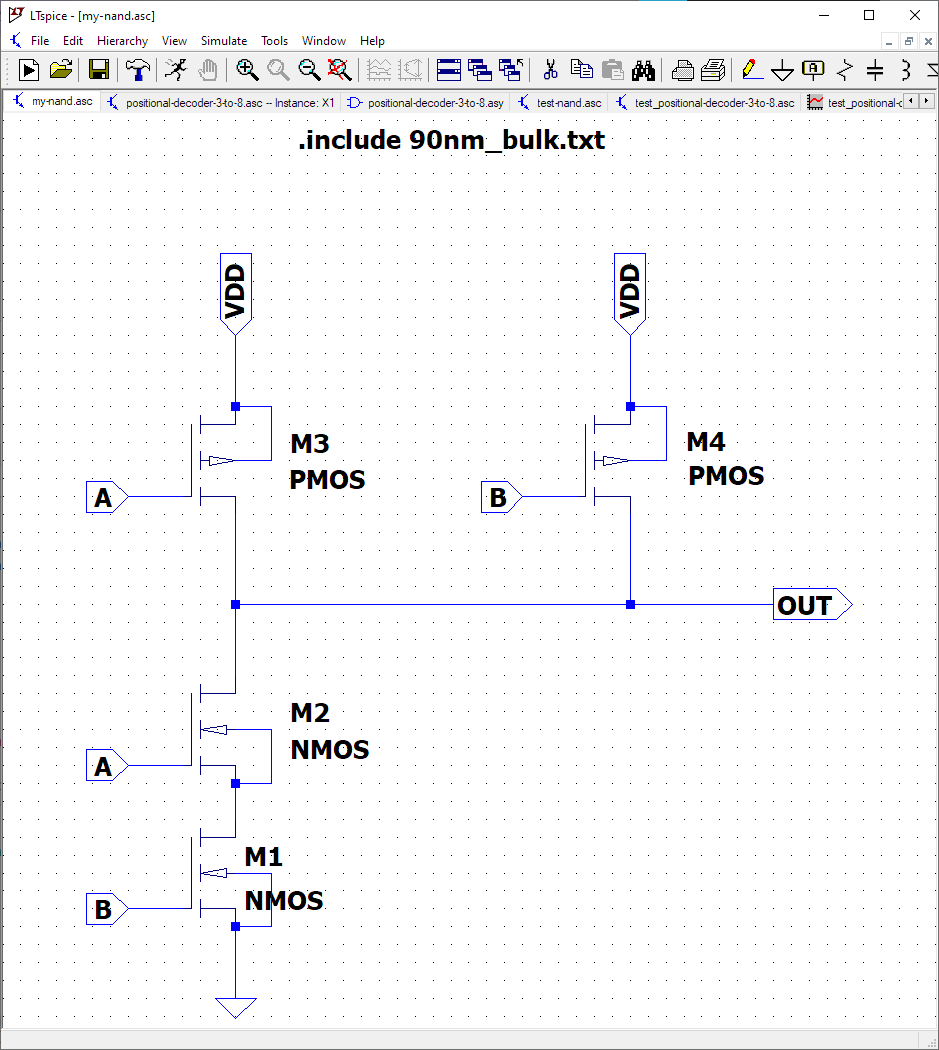
\includegraphics[width=0.6\textwidth]{res/nand_circuit.png}
%     \caption{Схема разработанного вентиля NAND.}
%     \label{fig:nand-circuit}
% \end{figure}
В элементе используется выделенный входной порт для питания VDD, чтобы
обеспечить независимость работы компонента от внутреннего элемента питания:
таким образом достигается установка глобального уровня сигнала соответствующего
логической единицы, с которым схема <<сравнивает>> входные сигналы. 
Так же для элемента NAND был разработан графический символ соответствующий
стандарту ANSI, его можно видеть на изображении \ref{fig:nand-symbol}.
\\
\begin{figure}[htb]
    \centering
    \begin{minipage}[b]{0.4\textwidth}
        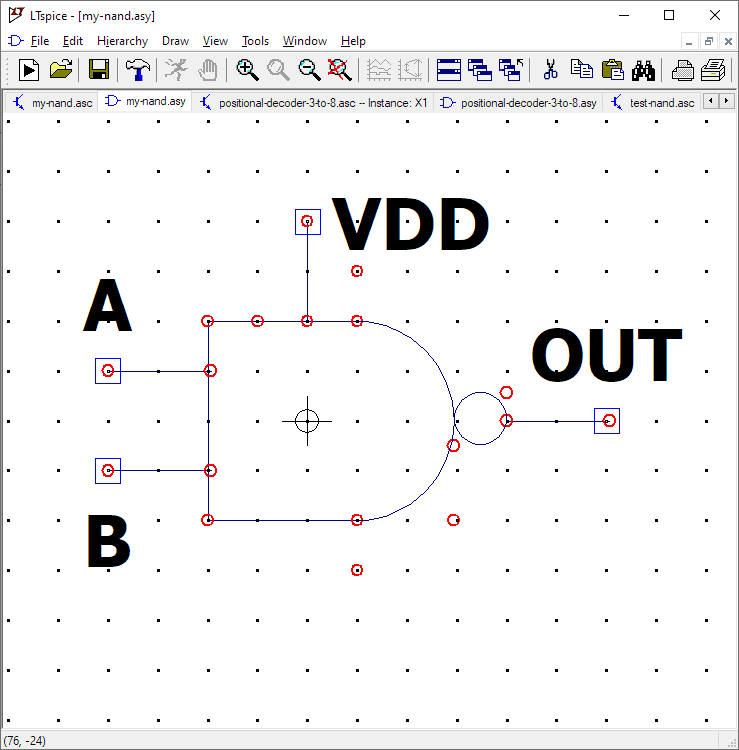
\includegraphics[width=\textwidth]{res/nand_symbol.png}
        \caption{Символ используемый для разработанного вентиля NAND.}
        \label{fig:nand-symbol}
    \end{minipage}
    \hfill
    \begin{minipage}[b]{0.5\textwidth}
        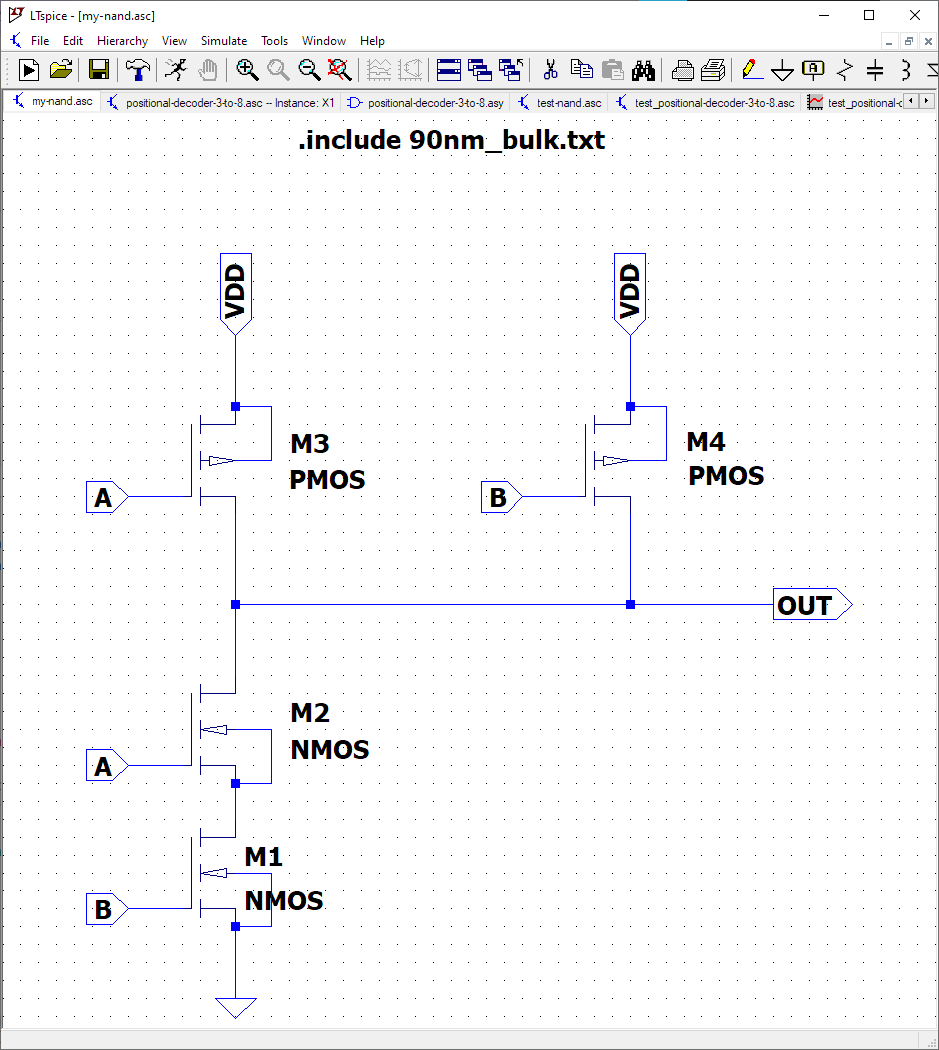
\includegraphics[width=\textwidth]{res/nand_circuit.png}
        \caption{Схема разработанного вентиля NAND.}
        \label{fig:nand-circuit}
    \end{minipage}
\end{figure}

Базисный логический элемент был протестирован с помощью схемы представленной на
изображении \ref{fig:nand-test}. 
\begin{figure}[htb]
    \centering
    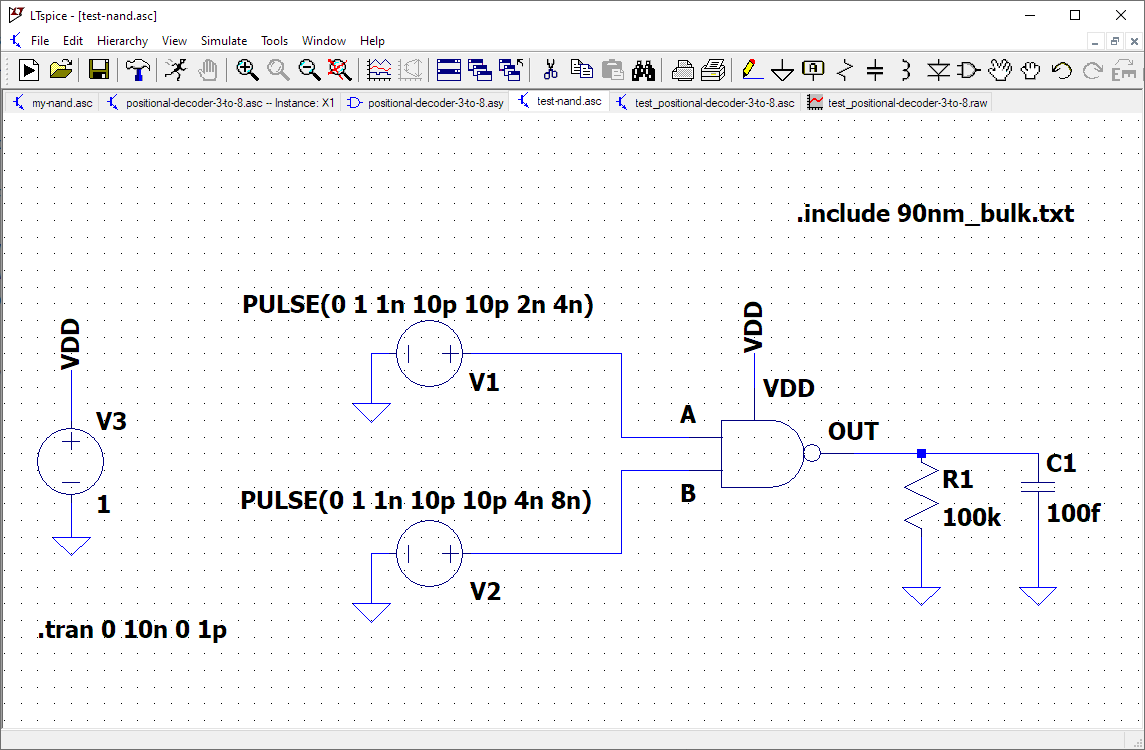
\includegraphics[width=\textwidth]{res/nand_test-circuit.png}
    \caption{Схема разработанная для тестирования компонента NAND.}
    \label{fig:nand-test}
\end{figure}
При этом, с целью пронаблюдать работу элемента NAND со всеми возможными
комбинациями входных значений во время симуляции, в схеме были использованы
импульсные элементы питания с различными периодами пульсации. А в качестве
нагрузки использовался резистор и конденсатора с характеристиками указанными в
задании.

Нагрузка представляет собой сопротивление обладающее как активным, так и
реактивным сопротивлением. Именно это сопротивление позволяет получить довольно
плавное изменение уровня выходного напряжения на элементе NAND и тем самым
достаточно качественно моделирует нагрузку в виде более сложной функциональной
схемы (зависимость уровня сигнала от характеристик нагрузки можно будет
наблюдать далее). 

%
Результат симуляции работы разработанной тестирующей схемы можно видеть на
изображении \ref{fig:nand-simulation} и более подробно с большим масштабом и
дополнительными обозначениями на изображении \ref{fig:nand-simulation-inspect}.
\begin{figure}[htb]
    \centering
    \begin{minipage}[b]{0.4\textwidth}
        \centering
        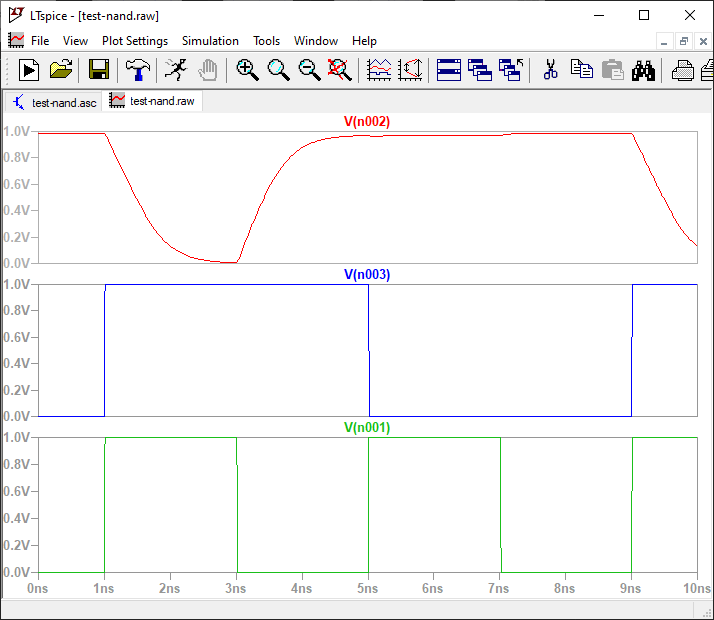
\includegraphics[width=\textwidth]{res/nand_simulation.png}
        \caption{Временная диаграмма симуляции работы тестирующей схемы для элемента NAND.}
        \label{fig:nand-simulation}
    \end{minipage}
    \hfill
% \end{figure}
% \begin{figure}[htb]
    \begin{minipage}[b]{0.55\textwidth}
        \centering
        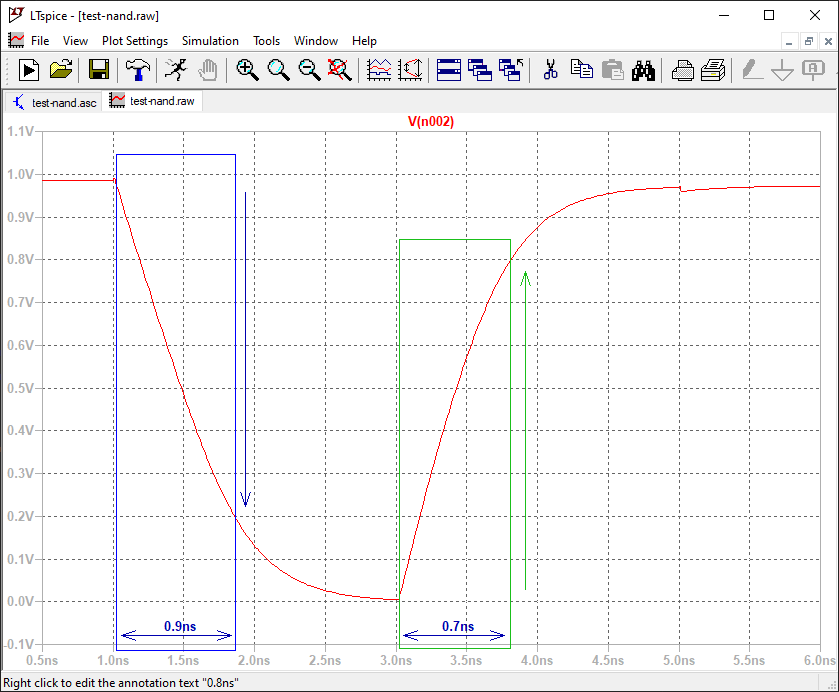
\includegraphics[width=\textwidth]{res/nand_simulation-inspect-level.png}
        \caption{Исследование временной диаграммы работы тестирующей схемы для элемента NAND на большем масштабе.}
        \label{fig:nand-simulation-inspect}
    \end{minipage}
\end{figure}

Для элемента NAND вычислим максимальную частоту для корректной его работы. Будем
считать, что логический высокий уровень начинается на значении 0,8 (В), а низкий
на значении 0,2 (В). Тогда, исходя из результатов моделирования
\ref{fig:nand-simulation-inspect}, длительность фронта сигнала и длительность
спада на декодере равны
$$T_{\mathrm{rise}} \approx 0,7 \text{ (нс) и}$$  
$$T_{\mathrm{fall}} \approx 0,9 \text{ (нс) }$$
соответственно, a длительность задержки тогда 
$$T_{\mathrm{delay}} = T_{\mathrm{rise}} + T_{\mathrm{fall}} = 1,6 \text{ (нс).}$$ 

Максимально допустимую частоту работы схемы можно определить по формуле
$$F_{\mathrm{max}} = \cfrac{1}{T_{\mathrm{delay}}} = 0,625 \text{ (ГГц).}$$
\\

Далее с использованием элемента NAND был построен БОЭ декодер, изображение схемы
которого можно видеть на изображении \ref{fig:decoder-circuit}. Для удобного его
проектирования использовались дополнительные порты для передачи инвертированных
значений входных сигналов. А для инверсии значения сигнала использовались компоненты NAND,
которым на оба входа подаются одинаковые значения --- так NAND вполне
компактно реализует логическую функцию NOT. 
\begin{figure}[!htb]
    \centering
    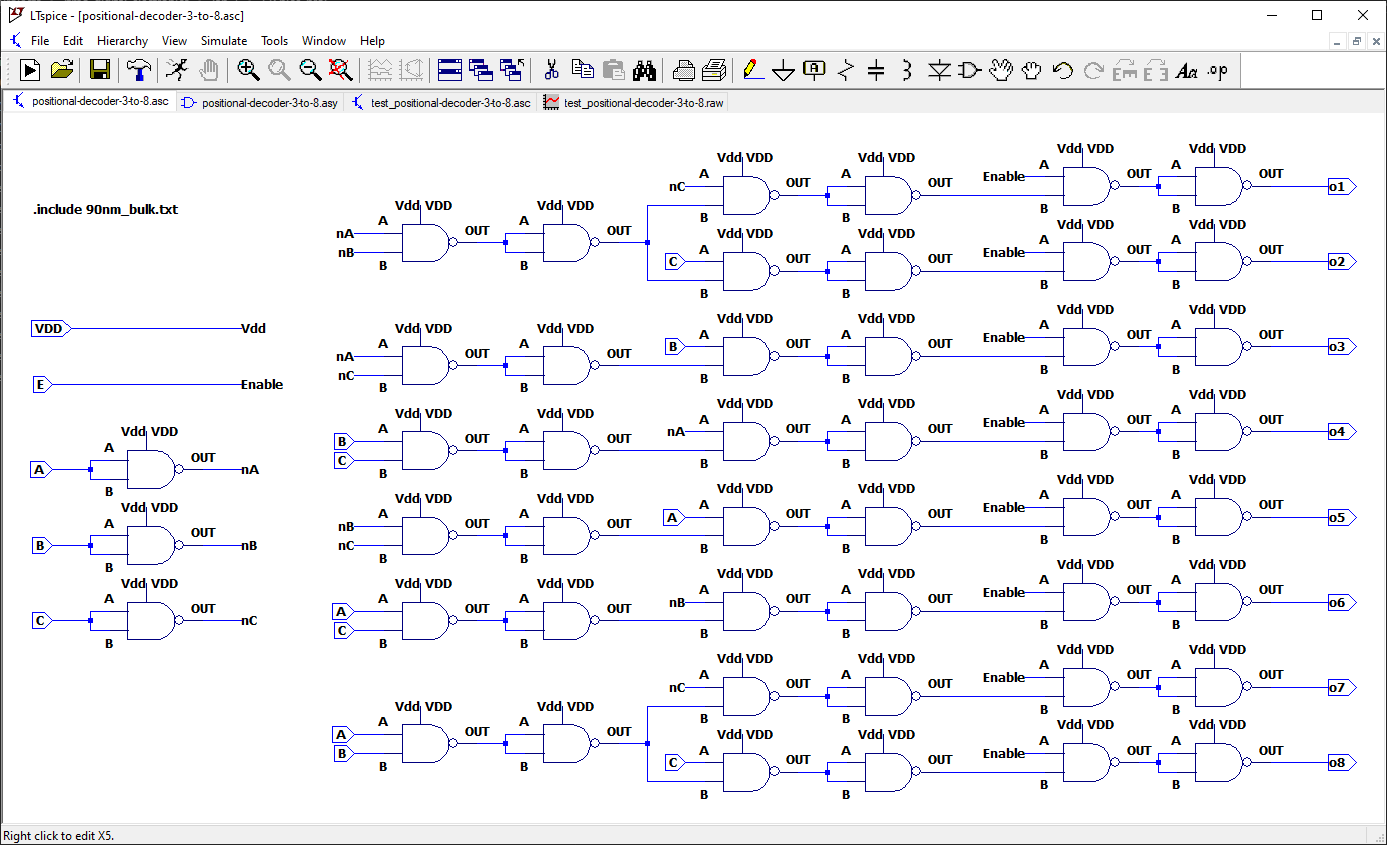
\includegraphics[width=\textwidth]{res/3-to-8-decoder_circuit.png}
    \caption{Схема разработанного позиционного декодера с использованием ранее разработанного логического базиса (NAND)}
    \label{fig:decoder-circuit}
\end{figure}

При разработке схемы использовалась идея, заключающаяся в том, что NAND дает на
выход значение, которое можно однозначно интерпретировать как комбинацию входных
значения только при условии, что оба входа поданы логические единицы: только в этом случае
можно использовать значение на выходе для определения состояния на обоих входах.

Также, изначально значение требуемого входного порта, отвечающего за включение
элемента (Enable), было ошибочно использовано как вход питания (логический высокий
уровень, Vdd) для элементов NAND, что обеспечивает нулевое значение на выходе
декодера в случае логического нуля на входе его питания, но в конечном итоге
пришли к выводу, что вход Enable должен отдельно контролировать поступление
входного сигнала на выход, а для питания NAND элементов в схему был добавлен еще один
входной порт, принимающий логический высокий уровень сигнала.

Для декодера был разработан графический символ, в котором 3 входных логических значения A, B, C и входное значение питания E. Внешний вид символа можно видеть на изображении \ref{fig:decoder-symbol}.
\begin{figure}[!htb]
    \centering
    \begin{minipage}[b]{0.3\textwidth}
        \centering
        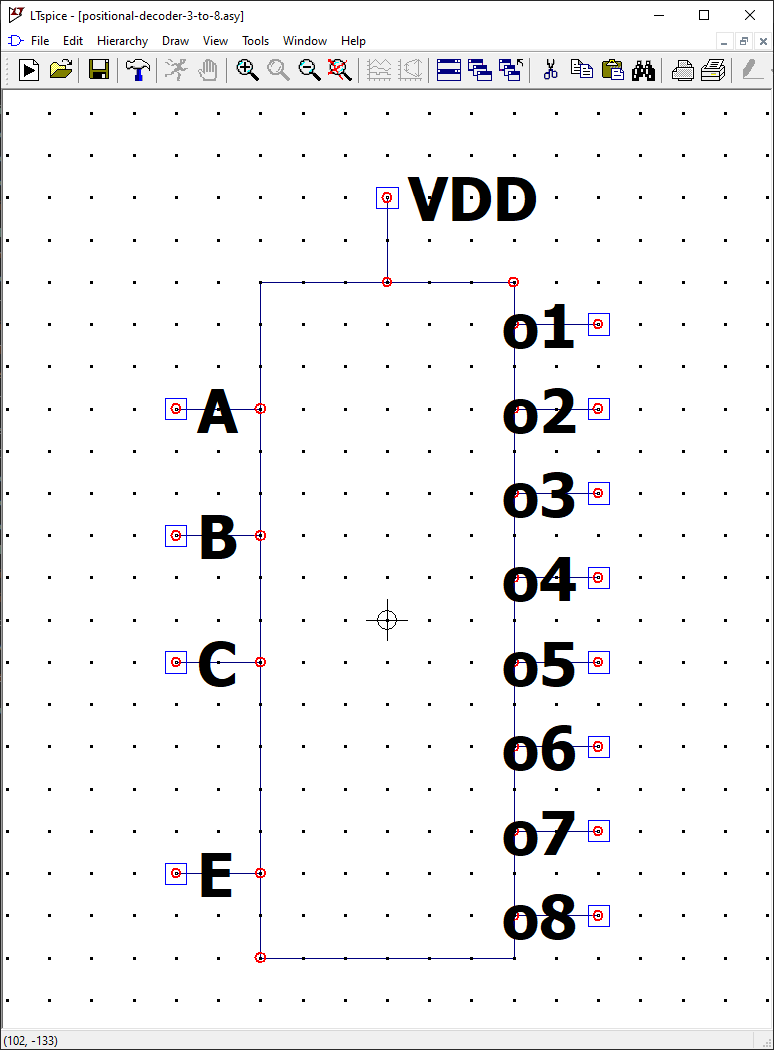
\includegraphics[width=\textwidth]{res/3-to-8-decoder_symbol.png}
        \caption{Символ позиционного декодера.}
        \label{fig:decoder-symbol}
    \end{minipage}
    \hfill
    \begin{minipage}[b]{0.65\textwidth}
        \centering
        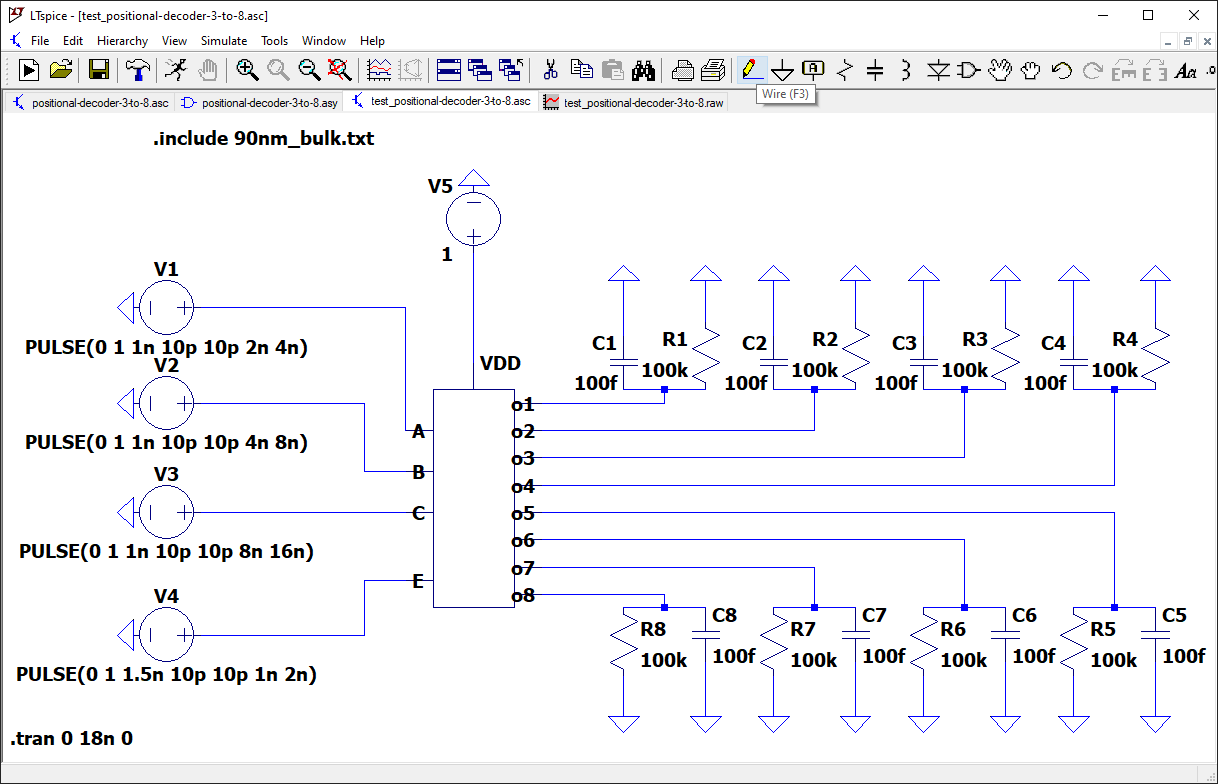
\includegraphics[width=\textwidth]{res/3-to-8-decoder_test-circuit.png}
        \caption{Схема для тестирования функциональности разработанного декодера.}
        \label{fig:decoder-test}
    \end{minipage}
\end{figure}
\\

Разработанный декодер был протестирован с использованием отдельной схемы,
представленной на изображении \ref{fig:decoder-test}. В ней на вход БОЭ
подавались значения с разных импульсных элементов питания, которые обладали
кратными периодами пульсации. Более того, элемент питания для входа E (Enable)
декодера тоже был  импульсным и при том со смещением периода относительно других
источников питания, чтобы продемонстрировать зависимость результата работы
декодера от этого входного сигнала. Каждый выходной порт декодера был подключен
к различному элементу нагрузки, чтобы исключить их замыкания. В качестве
нагрузки на компонент используются параллельно подключенные резистор и
конденсатор с характеристиками, указанными в условии лабораторной работы. 
% \begin{figure}[!htb]
%     \centering
%     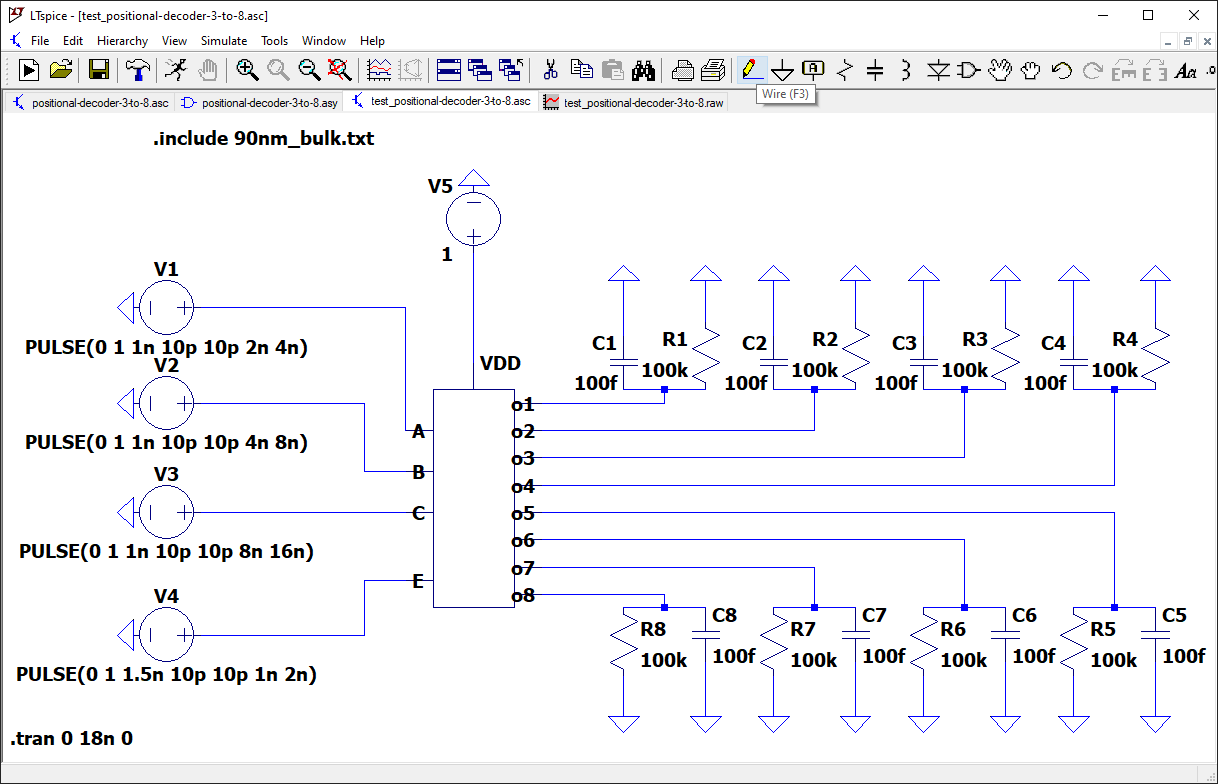
\includegraphics[width=\textwidth]{res/3-to-8-decoder_test-circuit.png}
%     \caption{Схема для тестирования функциональности разработанного декодера.}
%     \label{fig:decoder-test}
% \end{figure}

Во время симуляции работы декодера можно хорошо наблюдать изменение значений на
выходах декодера в разных комбинациях входных значений (см. графики на рисунке
\ref{fig:decoder-simulation}). При этом все изменения выходных значений
происходят строго в соответствии с входным значением Enable и так же им присущи
переходные процессы. 
\begin{figure}[!htb]
    \centering
    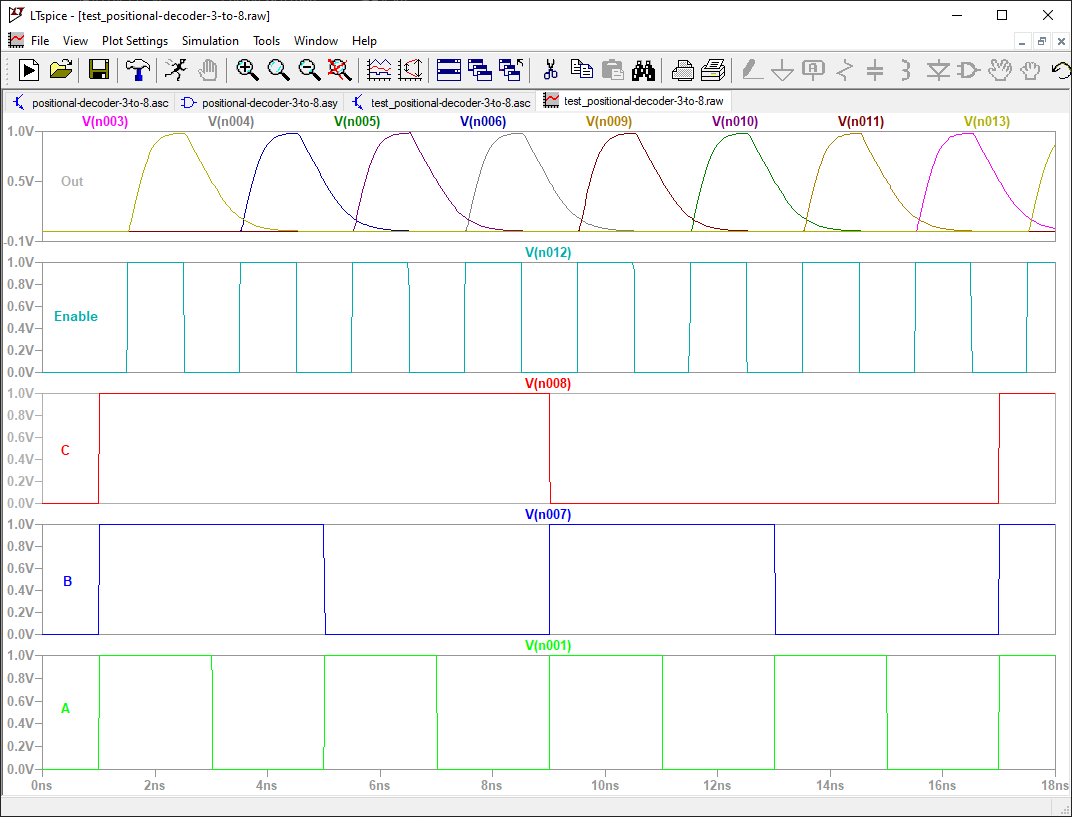
\includegraphics[width=\textwidth]{res/3-to-8-decoder_simulation.png}
    \caption{Временная диаграмма результата симуляции входных и выходных значений на разработанном декодере.}
    \label{fig:decoder-simulation}
\end{figure}

На временной диаграмме \ref{fig:decoder-simulation-inspect} симуляции можно
измерить задержки прохождения сигнала через схему БОЭ. 
\begin{figure}[!htb]
    \centering
    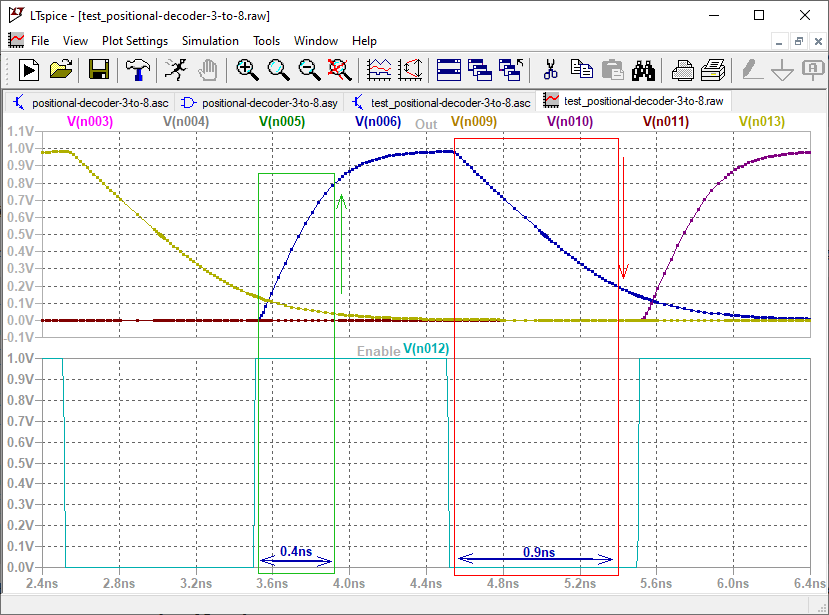
\includegraphics[width=0.8\textwidth]{res/3-to-8-decoder_simulation-inspect-level.png}
    \caption{Исследование временной диаграммы симуляции работы разработанного декодера на большем масштабе.}
    \label{fig:decoder-simulation-inspect}
\end{figure}
Изменения состояния будем считать, аналогично тому, как это делали для
логического элемента, т.е. 0,8 (В) --- верхний уровень, 0,2 (в) --- нижний. 
Тогда длительность фронта сигнала на декодере и длительность спада
$$T_{\mathrm{rise}} \approx 0,4 \text{ (нс) и}$$
$$T_\mathrm{fall} \approx 0,9 \text{ (нс)}$$
соответственно, а длительность задержки равняется
$$T_\mathrm{delay} = T_\mathrm{rise} + T_\mathrm{fall} = 1,3 \text{ (нс).}$$ 
Максимально допустимую частоту работы схемы можно определить по формуле 
$$F_\mathrm{max} = \cfrac{1}{T_\mathrm{delay}} \approx 0,77 \text{ (ГГц).}$$

Тут же можно заметить, что задержка фронта БОЭ (декодера) отличается от задержки
базисного элемента (NAND): 0,4 и 0,7 (нс) соответственно, а максимальная частота
для БОЭ больше чем для одного элемента. Считая, что среда разработки
симулирует верно, можно предположить, что уменьшение задержки вызвано именно сложной
комбинацией базисных элементов, что вызывает, к примеру, снижение общей
электроёмкости функционального компонента; активное сопротивление диодной схемы
при сложных соединениях практически не меняется. 

Для проверки этой теории был произведен тест с изменением ёмкости конденсатора в
нагрузке для конкретного выходного порта. На временной диаграмме симуляции, представленной на 
изображении \ref{fig:decoder-simulation-inspect-research}, можно видеть, что при
увеличении ёмкости конденсатора в нагрузке, задержка фронта увеличивается
приблизительно до ожидаемого значения 0,7 (нс), но также меняется форма сигнала.
Похоже, что при достижении нужного соотношения между ёмкостями функциональных
элементов задержки принимают определенные значения. (как позже окажется, это не
вполне верное замечание)
\begin{figure}[H]
    \centering
    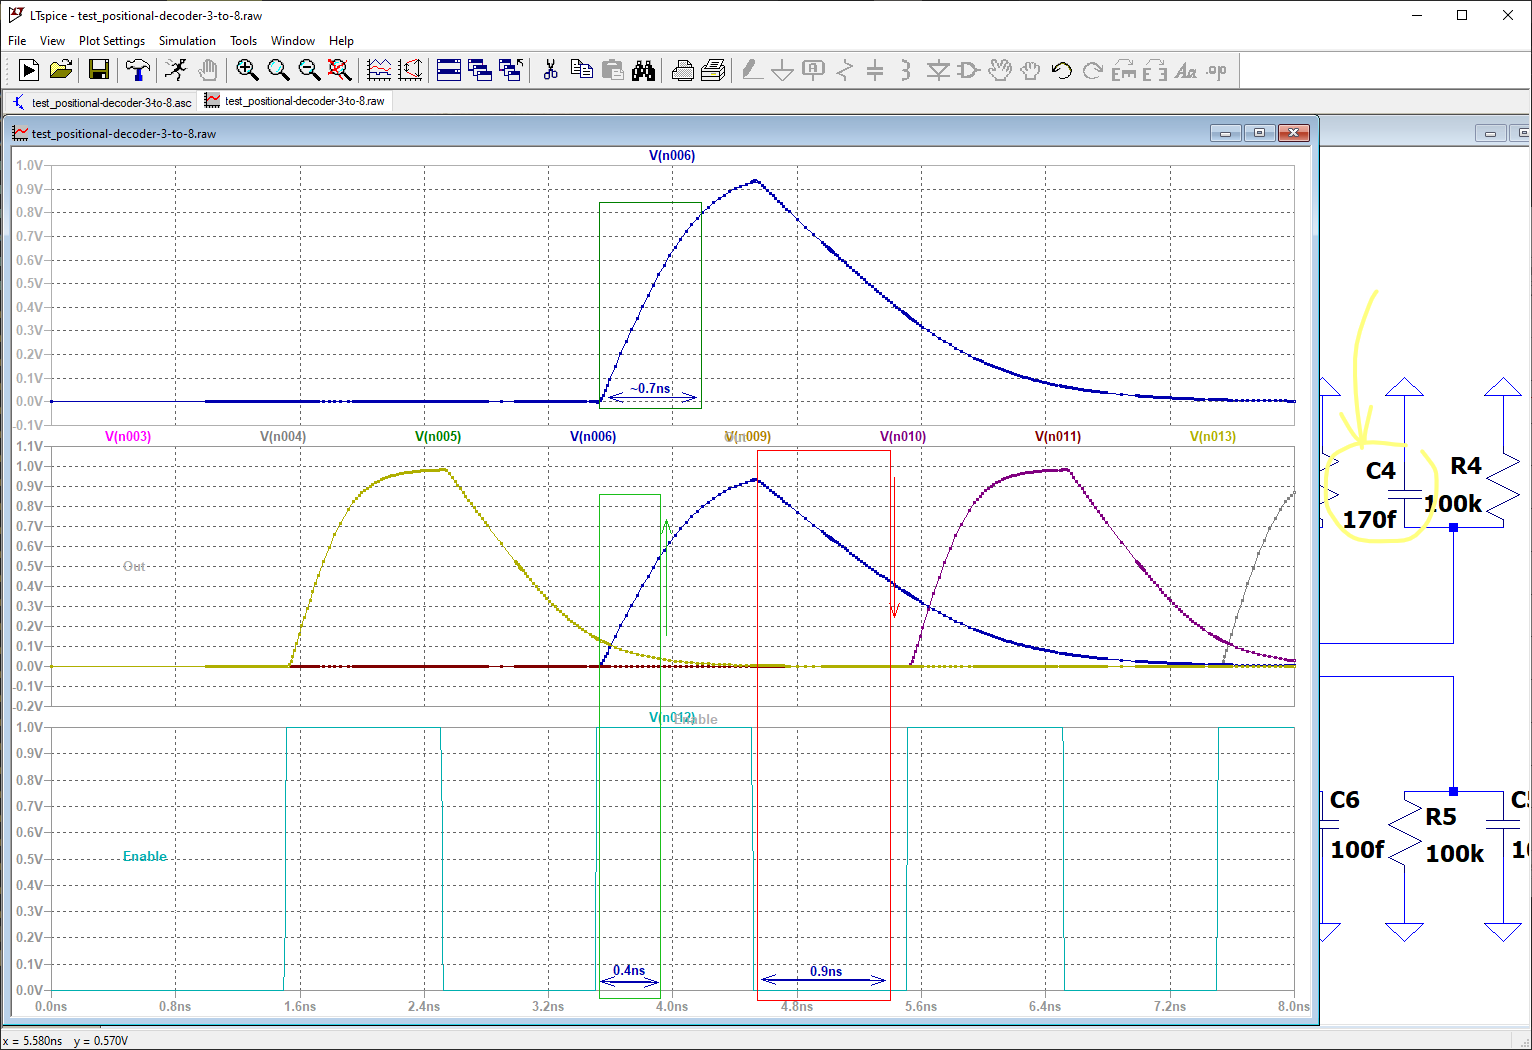
\includegraphics[width=0.8\textwidth]{res/3-to-8-decoder_simulation-inspect-level-research.png}
    \caption{Исследование временной диаграммы симуляции с измененными характеристиками нагрузки.}
    \label{fig:decoder-simulation-inspect-research}
\end{figure}

Во время защиты лабораторной, пришли к умозаключению, что на
на деле измеряются не задержки на БОЭ, а время зарядки конденсатора в нагрузке.

\Subsection{Часть 2: описание схемы в Vivado}

В соответствии с заданием был разработан программный модуль описывающий работу
БОЭ (декодера 3 в 8), см. листинг \ref{lst:decoder-verilog}. При его реализации
в качестве базисных логических элементов так же использовались NAND компонента,
но на в этом случае программная среда предоставляет его без необходимости
реализовывать самому. В добавок к этому, можно наблюдать значительное отличие
метода описания функциональной схемы кодом от составления графической схемы ---
программная среда сама заботится о передаче в компоненты низкого и высокого
логического уровня сигнала, поэтому элементы \verb|nand| имеют всего 3
аргумента: выходной порт и два входных. 

Для реализации модуля была использована идея аналогичная реализации БОЭ в LTSpice,
только теперь потребовалось использовать несколько дополнительных соединительных 
проводов (шин), как бы, обозначающих вертикальное сечение схемы. Важно заметить,
что в реализации используется определенный порядок бит в выходном проводе, чтобы 
значение на выходе правильным образом соответствовали численному значению.
\\

\lstinputlisting[language=verilog,caption={Код программного модуля реализующего логику треуемого БОЭ, декодера 3 в 8},label={lst:decoder-verilog}]{res/decoder.v}

Также в соответствии с заданием был разработан программный модуль, тестирующий
логику ранее разработанного БОЭ, см. листинг \ref{lst:decoder-tb-verilog}. Там
для тестирования используется модуль реализующий логику требуемого декодера, но
с помощью высокоуровневых средств языка Verilog, его код можно видеть на
листинге \ref{lst:decoder-golden-verilog}. Он выступает в роли <<золотого
стандарта>>, который не нужно тестировать. С ним следует сравнивать результат
работы компонента реализованного с помощью логического базиса, чтобы
удостовериться в корректности работы схемы.
\\
 
\lstinputlisting[language=verilog,caption={Код программного модуля тестирующего логику позиционного декодера 3 в 8},label={lst:decoder-tb-verilog}]{res/decoder_tb.v}

\lstinputlisting[language=verilog,caption={Код программного модуля реализующего логику позиционного декодера 3 в 8 с помощью высокоуровневых возможностей языка Verilog},label={lst:decoder-golden-verilog}]{res/decoder_golden.v}

В тестовом модуле изначально проверялось, что в цикле для всех возможных входных
значений, подаваемых на вход сигналов, (соответствующих двоичному представлению
чисел от 0 до 7) на выход подавались сигналы, соответствующие двоичному
представлению числа 2 в степени входного двоичного числа. Иными словами,
логическая 1 должна быть выставлена на порт с номером, равным 2 в степени
входного двоичного числа. Это производилось с помощью оператора возведения в
степень в языке Verilog (\verb|2**i|).

Позже тест был переписан с использованием дополнительного модуля. Теперь в тесте
просто сравнивается выходное значение с <<доверенного>> компонента и
тестируемого. В случае соответствия работы компонента поставленным требованиям,
на экран выводится сообщение о корректности работы для конкретной комбинации
сигналов; в противном случае --- сообщение о некорректности работы и ожидаемом
значении.
\\


Еще в среде разработки Vivado была получена временная диаграмма симуляции работы
разработанного компонента, её можно видеть на изображении
\ref{fig:decoder-vivado-symulation}. Как и ожидалось, сигналы имеют определенные
в программе значения и тестируемый модуль соответствует работе тестирующего
модуля.

\begin{figure}[H]
    \centering
    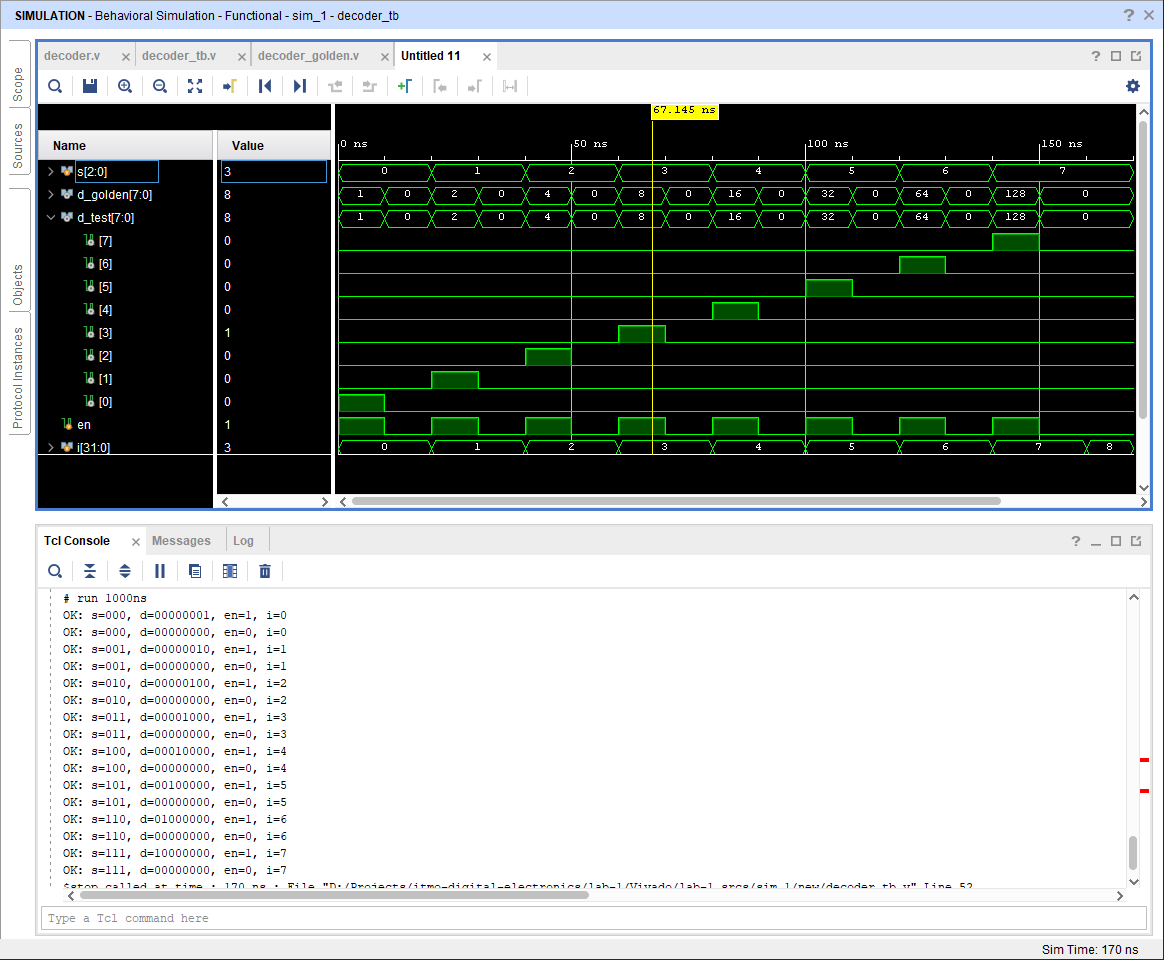
\includegraphics[width=\textwidth]{res/3-to-8-decoder_vivado-simulation.png}
    \caption{Временная диаграмма симуляции работы БОЭ в тестовом окружении в среде Vivado}
    \label{fig:decoder-vivado-symulation}
\end{figure}

\Section{Вывод}

В рамках выполнения работы были выполнены все поставленные задачи. Были
приобретены навыки разработки цифровых схем в приложении LTSpice с последующей
симуляцией их работы. Главной сложностью при этом стало понять логику
комбинирования функциональных компонентов: для меня было не очевидно, что сигнал
<<питания>> и сигнал высокого логического уровня не совпадают. Оказалось, что
для более точной физической реализации, каждый компонент должен быть подключен
независимо к линии с высоким логическим уровнем напряжения. Также было видно, насколько
выбор логического базиса влияет на сложность составления БОЭ, мне удалось наблюдать, как
другим учащимся было тяжело составить свою схему с помощью других базисных элементов.

В то же время, среда разработки Vivado и в частности язык Verilog позволяют избавиться от муторного и сложного управления подключением линий сигнала логических 1 и 0. Вместо этого Verilog позволяет описывать логику взаимодействия компонентов без погружения в детали физического устройства компонентов. 

Отдельное впечатление оставляет способ дистрибуции среды Vivado: 20 (ГБ) образ
для версии 2019 года --- это что-то с чем-то. Более того на сайте производителя
эта система поставляется образами по 100 с лишним гигабайт, что заставляет
задуматься о внутреннем устройстве этой системы, ведь внешний вид у нее не
блещет изяществом, и требованиям к средствам разработки реальных вычислительных
систем. Вероятно это приложение содержит в себе огромное количество
дополнительных драйверов для работы с разными типами устройств. Ярко видно
различие сред разработки обычных программных систем и разработки физических
вычислительных систем.

Самый важный вывод, который можно сделать при выполнении лабораторной работы,
был получен во время ее защиты. Как можно было заметить, форма сигнала
получаемая в LTSpice при модулировании, зависит от параметров нагрузочных
конденсаторов. Стало быть, на самом деле в схеме происходит измерение не задержек 
на БОЭ, а времени зарядки нагрузочных конденсаторов. Паразитические ёмкости
диодов значительно меньше даже таких маленьких емкостей конденсаторов данных в
задании, поэтому в таких реалиях нет возможности корректно измерить задержки на
БОЭ и только при очень маленькой (в идеале нулевой) внешней емкости получится
увидеть время задержки БОЭ кратное времени задержки внутренних элементов.



% Вывод... 
% Ссылка на источники \cite{itmocompmath}.
% -- из biblist
% Прямая ссылка на интернет-ресурс: \href{https://http.cat/501}{http.cat}
% \newpage
%<<<<<<<<<<<<<<<<<<<<<< КОД РАБОТЫ <<<<<<<<<<<<<<<<<<<<<<<<


%>>>>>>>>>>>>>>>> СПИСОК ЛИТЕРАТУРЫ >>>>>>>>>>>>>>>>>>>>>>>
% \include{biblist}  % Для соответсвия гост, придется доработать. Нужен файл .bib
%<<<<<<<<<<<<<<<<<<<< СПИСОК ЛИТЕРАТУРЫ <<<<<<<<<<<<<<<<<<<


\end{document}
%<<<<<<<<<<<<<<<< ,,,,,,,,,,,,,,,,,,,,,,, <<<<<<<<<<<<<<<<<
%<<<<<<<<<<<<<<<<<<< СОДЕРЖИМОЕ ОТЧЕТА <<<<<<<<<<<<<<<<<<<<
